%Book
%Copyright (C) 2019  Patrick Diehl
%
%This program is free software: you can redistribute it and/or modify
%it under the terms of the GNU General Public License as published by
%the Free Software Foundation, either version 3 of the License, or
%(at your option) any later version.

%This program is distributed in the hope that it will be useful,
%but WITHOUT ANY WARRANTY; without even the implied warranty of
%MERCHANTABILITY or FITNESS FOR A PARTICULAR PURPOSE.  See the
%GNU General Public License for more details.

%You should have received a copy of the GNU General Public License
%along with this program.  If not, see <http://www.gnu.org/licenses/>.

% The template of the book is based on the The Legrand Orange Book
% LaTeX Template
% Version 2.4 (26/09/2018)
% Original author:
% Mathias Legrand (legrand.mathias@gmail.com) with modifications by:
% Vel (vel@latextemplates.com)
% License:
% CC BY-NC-SA 3.0 (http://creativecommons.org/licenses/by-nc-sa/3.0/)

%----------------------------------------------------------------------------------------
%	PACKAGES AND OTHER DOCUMENT CONFIGURATIONS
%----------------------------------------------------------------------------------------

\documentclass[11pt,fleqn]{book} % Default font size and left-justified equations

\input{structure.tex} % Insert the commands.tex file which contains the majority of the structure behind the template

\hypersetup{pdftitle={Parallel Computational Mathematics},pdfauthor={Patrick Diehl, Phd}} % Uncomment and fill out to include PDF metadata for the author and title of the book

%----------------------------------------------------------------------------------------

\begin{document}

%----------------------------------------------------------------------------------------
%	TITLE PAGE
%----------------------------------------------------------------------------------------

\begingroup
\thispagestyle{empty} % Suppress headers and footers on the title page
\begin{tikzpicture}[remember picture,overlay]
%\node[inner sep=0pt] (background) at (current page.center) {\includegraphics[width=\paperwidth]{background.pdf}};
\draw (current page.center) node [fill=azure!30!white,fill opacity=0.6,text opacity=1,inner sep=1cm]{\Huge\centering\bfseries\sffamily\parbox[c][][t]{\paperwidth}{\centering Parallel Computaitonal Mathematics\\[15pt] % Book title
{\Large Fall 2020}\\[20pt] % Subtitle
{\huge Dr. Patrick Diehl}}}; % Author name
\end{tikzpicture}
\vfill
\endgroup

%----------------------------------------------------------------------------------------
%	COPYRIGHT PAGE
%----------------------------------------------------------------------------------------

\newpage
~\vfill
\thispagestyle{empty}

\noindent Copyright \copyright\ 2020 Patrick Diehl\orcid{0000-0003-3922-8419}\\ % Copyright notice

%\noindent \textsc{Published by Publisher}\\ % Publisher

\noindent \url{https://www.cct.lsu.edu/~pdiehl/teaching/2020/4997/}\\ % URL

\noindent \doclicenseThis  

\noindent \textit{Edition, Fall 2020} % Printing/edition date

%----------------------------------------------------------------------------------------
%	TABLE OF CONTENTS
%----------------------------------------------------------------------------------------

%\usechapterimagefalse % If you don't want to include a chapter image, use this to toggle images off - it can be enabled later with \usechapterimagetrue

%\chapterimage{chapter_head_1.pdf} % Table of contents heading image

\pagestyle{empty} % Disable headers and footers for the following pages

\tableofcontents % Print the table of contents itself

\cleardoublepage % Forces the first chapter to start on an odd page so it's on the right side of the book

\pagestyle{fancy} % Enable headers and footers again

\chapter*{Forward}

%----------------------------------------------------------------------------------------
%	PART
%----------------------------------------------------------------------------------------

\part{Introduction: C++ and the C++ standard template library}

%----------------------------------------------------------------------------------------
%	CHAPTER 1
%----------------------------------------------------------------------------------------

%\chapterimage{chapter_head_2.pdf} % Chapter heading image

%----------------------------------------------------------------------------------------
\chapter{Introduction C++}
%----------------------------------------------------------------------------------------
This chapter gives a brief introduction to the core features of the C++ language. However, the focus on this chapter is to introduce the C++ standard template library, see Section~\ref{chapter:stl}, which is essential to implement mathematical equations and algorithms. Therefore, we quickly look into these features as we need them to implement the numerical examples in Part~\ref{part:numerical:examples}. For more details we refer to
\begin{itemize}
\item \fullcite{andrew2000accelerated}
\end{itemize}
since this book gives an excellent pragmatic overview with a lot of examples. For even more C++ basics, we refer to
\begin{itemize}
\item \fullcite{stroustrup2014programming}.
\end{itemize}
%----------------------------------------------------------------------------------------
\section{History of C and C++}
%----------------------------------------------------------------------------------------

%----------------------------------------------------------------------------------------
\section{Getting started with C++}
%----------------------------------------------------------------------------------------
To begin with C++ programming, we look at a simple C++ program, the so-called ``Hello World'' example which most programming language start with. Listing~\ref{code:hello:world} shows this program and the first line in green a comment is shown. A  single-line comments always starts with \lstinline[language=C++]|//| and is used to explain the functionality of the program or the next lines of codes. It is also possible to use multi-line comments\endnote{\url{https://en.cppreference.com/w/cpp/comment}} by using \lstinline[language=C++]{/* */}. Comments are important to understand the program, especially if the code is shared with other collaborators. Fore more details we refer to~\cite{kernighan1974elements}.

The second line starts with a so-called include directive\endnote{\url{https://en.cppreference.com/w/cpp/preprocessor/include}} \lstinline[language=C++]{#include <iostream>}. This include directive is needed to include functionality of the C++ standard library, see Chpater~\ref{chapter:stl}, in our case we include the \lstinline|iostream| header to print the Hello World to the terminal, see Line 6.

The fourth line \lstinline[language=C++]{int main()} starts with the so-called Main function\endnote{\url{https://en.cppreference.com/w/cpp/language/main_function}} which is the entry point of the program and all code lines within are executed sequentially one by one. Every C++ which will be compiled to an executable needs exact one function called \lstinline[language=C++]|main| which have a integer \lstinline[language=C++]{int} as its return type. On most operation systems a return value of zero means that the program executed successfully and any other value indicates an failure. The second last line \lstinline[]|return| is the so--called return statement\endnote{\url{https://en.cppreference.com/w/cpp/language/return}} which has to match the return type in front of the \lstinline[language=C++]{int main()}.


\lstinputlisting[language=C++,caption={A simple C++ program, the so-called ``Hello World'' example, which most languages start with.\label{code:hello:world}},float,floatplacement=h]{ParallelComputationMathExamples/chapter2/lecture1-main.cpp}

Once we have written the program, we have to compile the C++ code into an executable to run the code and print ``Hello world'' to the terminal. Note that there are plenty of C++ compilers\endnote{\url{https://en.wikipedia.org/wiki/List_of_compilers\#C++_compilers}} available, however this book will use the GNU Compiler Collection (GCC) for all examples. Line 1 in Listing~\ref{code:hello:world:compile} shows how to compile the file \lstinline[language=bash]|lecture1-1.cpp|, which contains the C++ code in Listing~\ref{code:hello:world}, to an executable. The GCC provides the \lstinline[language=bash]{g++} compiler to compile C++ code and the \lstinline[language=bash]{gcc} compiler to compile C code. As the first argument to the \lstinline[language=bash]{g++} compiler the file name of the C++ is provided and with the \lstinline[language=bash]|-o| option the name of the executable is specified. To run the generated executable, we type \lstinline[language=bash]|./lecture-1-1| in the terminal. Note for the basic usage of the Linux terminal we refer to~\cite{newham2005learning,robbins2016bash}.

\lstinputlisting[language=bash,caption={Compilation and execution of the C++ program.\label{code:hello:world:compile}},float,floatplacement=h,firstline=2, lastline=3]{ParallelComputationMathExamples/chapter2/lecture1-main.sh}

\begin{exercise}
Download the example program\endnote{\url{https://github.com/diehlpkteaching/ParallelComputationMathExamples}} from GitHub and compile it with your favorite C++ compiler. After you ran the example you could try to modify it, for example you could print a different text or add a second line to the output.
\end{exercise}


%----------------------------------------------------------------------------------------
\section{Fundamental data types}
%----------------------------------------------------------------------------------------
\index{data types!fundamental}
In this section the fundamental data types\endnote{\url{https://en.cppreference.com/w/cpp/language/types}} provided by the C++ language are introduced. First, the numeric data types are introduced. To represent natural numbers $\mathbb{N}=\{0,1,2,\ldots \}$ the \lstinline[language=C++]|unsigned int| data type is available. To represent integer numbers $\mathbb{Z}=\{\ldots,-2,-1,0,1,2,\ldots \}$ the \lstinline[language=C++]|int| data type is available. For all these data types following options: \lstinline[language=C++]|short|, \lstinline[language=C++]|long|, and \lstinline[language=C++]|long long| are available. For more details about the binary numeral system we refer to~\cite{gilli1965binary}. To represent real numbers $\mathbb{R}$ the \lstinline[language=C++]|float| data type and \lstinline[language=C++]|double| data type are available. Fore more details about the IEEE 474 standard how floating point numbers are represented in the computer we refer to~\cite{4610935,goldberg1991every}. Table~\ref{chapter2:table:datatypes} summarizes all the available numeric data types and there ranges. The next section shows how to get the range of the IEEE 474 standard how floating point numbers.

\begin{table}[h]
\centering
\begin{tabular}{lccc}
\toprule
Data type & Size (Bytes) & Min & Max \\\midrule
\multicolumn{4}{c}{Natural numbers $\mathbb{N}$ }\\\midrule
\lstinline[language=C++]|unsigned short int| & 2 & 0 & 65,535  \\ 
\lstinline[language=C++]|unsigned int| & 4 & 0 & 4,294,967,295 \\ 
\lstinline[language=C++]|unsigned long int| & 4 & 0 & 4,294,967,295 \\ 
\lstinline[language=C++]|unsigned long long int| & 8 & 0 & 8,446,744,073,709,551,615 \\ \midrule
\multicolumn{4}{c}{Integer numbers $\mathbb{Z}$ }\\\midrule
\lstinline[language=C++]|short int| & 2 & -32,768 & 32,768 \\
\lstinline[language=C++]|int| & 4 & -2,147,483,648 & 2,147,483,648 \\
\lstinline[language=C++]|long long int| & 8 & $-2^{63}$ & $2^{63}-1$ \\\midrule
\multicolumn{4}{c}{Real numbers $\mathbb{R}$ }\\\midrule
\lstinline[language=C++]|float| & 4 &  &  \\
\lstinline[language=C++]|double| & 8 &  &  \\
\bottomrule
\end{tabular} 
\caption{Overview of the fundamental numeric data types.}
\label{chapter2:table:datatypes}
\end{table}

To represent a boolean value $\mathbf{B}=\{0,1\}$ the \lstinline[language=C++]|bool| data type which has either one of the two values \lstinline[language=C++]|true| or \lstinline[language=C++]|false|. Note that the C++ STL offers \lstinline|std::complex|\endnote{\url{https://en.cppreference.com/w/cpp/numeric/complex}} for complex number $\mathbb{C}$, however, this one is not within the fundamental data types.

%----------------------------------------------------------------------------------------
\section{Statements and flow control}
%----------------------------------------------------------------------------------------

%----------------------------------------------------------------------------------------
\subsection{Iteration statements}
\label{sec:iteration:statements}
%----------------------------------------------------------------------------------------
\index{statements!iteration} For some applications, we have to repeat some operations multiple times. The C++ language provides the so-called iteration statements. There are two iteration statements, the \lstinline[language=C++]|for| loop and the \lstinline[language=C++]|while| loop, respectively. Let us look how to compute the sum of the numbers from one up ton $n$
\begin{align}
r = \sum\limits_{i=1}^n i\text{.}
\end{align}
The first option is using a \lstinline[language=C++]|for| loop statement\endnote{\url{https://en.cppreference.com/w/cpp/language/for}}\index{loop!for statement} which shown in Listing~\ref{code:for:loop}. Line 9 shows the \lstinline[language=C++]|for| loop statement with its three arguments. First, the so--called loop variable \lstinline[language=C++]{size_t i = 0} which is initialized to zero. Note that the loop variable is only defined within the loop's body (The part between the curly braces). Second, the so--called condition statement \lstinline[language=C++]{i < n} which means that the loop body is repeated until the variable $i$ is larger than $n$. The third statement manipulates the loop variable, in our case the loop variable is incremented by one after the loop body was executed once. Note that we use the \lstinline[language=C++]|for| loop statement, if we know how often we have to loop through the loop body in advance.


\lstinputlisting[language=C++,caption={Computation of the sum from one up to $n$ using the for loop statement. \label{code:for:loop}},float,floatplacement=h]{ParallelComputationMathExamples/chapter2/lecture1-for.cpp}

The second option is using a \lstinline[language=C++]|while| loop statement\endnote{\url{https://en.cppreference.com/w/cpp/language/while}}\index{loop!while statement} which shown in Listing~\ref{code:while:loop}. Line 10 shows the \lstinline[language=C++]|while| loop statement with its one argument. This is the so-called condition statement  \lstinline[language=C++]{i < n} which means that the loop body is repeated until the variable $i$ is larger than $n$. Note in the previous example we had three arguments. Here, the loop variable is declared before the loop in Line 9 and the third statement is  in Line 13 where the loop variable is incremented by one in each iteration. Note that we use the \lstinline[language=C++]|while| loop statement, if we do not know the amount of iterations in advance. This example has shown that we can write every \lstinline[language=C++]|for| loop statement as a \lstinline[language=C++]|while| loop statement. For more details we refer to~\cite[Chapter~2]{andrew2000accelerated}.   


\lstinputlisting[language=C++,caption={Computation of the sum from one up to $n$ using the while loop statement..\label{code:while:loop}},float,floatplacement=h]{ParallelComputationMathExamples/chapter2/lecture1-while.cpp}

\begin{exercise}
Define in your own words in which case you should use a \lstinline[language=C++]|for| loop statement and a \lstinline[language=C++]|while| loop statement. 
\end{exercise}

%----------------------------------------------------------------------------------------
\subsection{Selection statements}
%----------------------------------------------------------------------------------------
\index{statements!selection}
For some applications, we have to select different behavior of the code depending on conditions. Equation~\ref{eq:chapter2:if} shows how to compute the sum from one to $n$ with different cases for even and odd numbers, If the number is even the number keeps the same and for odd numbers the number is squared.
\begin{align}
r = \sum\limits_{i=1}^n f(i) \text{  with  } f(i) = 
\begin{cases}
i, \text{ if } i \text{ is even} \\
i^2, \text{ else}
\end{cases}
\label{eq:chapter2:if}
\end{align}
Listing~\ref{code:example-if} shows the implementation of Equation~\ref{eq:chapter2:if} using a \lstinline[language=c++]{for} loop. The skeleton of the \lstinline[language=c++]{for} loop is identical to the one in Listing~\ref{code:for:loop}, but the \lstinline[language=c++]{if} statement\endnote{\url{https://en.cppreference.com/w/cpp/language/if}} in Line 8 is added to switch between even and odd numbers. The \lstinline[language=c++]{if} statement takes exactly one argument, the so--called condition statement. If the statement is evaluated as \lstinline[language=c++]{true} the code line between \lstinline[language=c++]{if} and \lstinline[language=c++]{else} is selected.  If the statement is evaluated as \lstinline[language=c++]{false} the code line after \lstinline[language=c++]{else} is selected. Multiple lines of codes have to be between curly braces. It is also possible to use \lstinline[language=c++]{else if} after the first \lstinline[language=c++]{if}. \\

\lstinputlisting[language=C++,caption={Computation of the sum from one up to $n$ using the selection statement.\label{code:example-if}},float,floatplacement=h]{ParallelComputationMathExamples/chapter2/lecture1-if.cpp}


The second selection statement is the \lstinline[language=c++]{switch} statement\endnote{\url{https://en.cppreference.com/w/cpp/language/switch}}. For example this statement can be used to execute different code branches depending on a single variable. Listing~\ref{code:example-switch} shows one example to write the name of the color to the standard output. In this case we use a enumeration \lstinline[language=c++]{enum}\endnote{\url{https://en.cppreference.com/w/cpp/language/enum}} to store the colors. The \lstinline[language=c++]{switch} takes one argument and execute the code between the matching \lstinline[language=c++]{case} and the following \lstinline[language=c++]{break}.


\lstinputlisting[language=C++,caption={Computation of the sum from one up to $n$ using the selection statement.\label{code:example-switch}},float,floatplacement=h]{ParallelComputationMathExamples/chapter2/lecture1-switch.cpp}


%----------------------------------------------------------------------------------------
\subsection{Operators}
%----------------------------------------------------------------------------------------
\index{Operators}
For the example in Listing~\ref{code:for:loop} we have seen the operator \lstinline[language=C++]|i<n| which is a so--called comparison operator. Next to the comparison operators, C++ language has following operators\endnote{\url{https://en.cppreference.com/w/cpp/language/operator_precedence}}:
\begin{itemize}
\item Comparison operators, see Table~\ref{sec:1:tab:operator:comp},
\item Arithmetic operators, see Table~\ref{sec:1:tab:operator:arithmetic},
\item Logical operators, see Table~\ref{sec:1:tab:operator:logical}, and
\item Assignment operators, see Table~\ref{sec:1:tab:operator:assign},
\end{itemize}
 logical operators, arithmetic, and assignment.

\begin{table}[p]
\centering
\begin{tabular}{clll}
\toprule
Operator & Name  & Example \\ 
\midrule
\lstinline|==| & Equal to & \lstinline|x==y|\\ 
\lstinline|!=| & Not equal & \lstinline|x!=y|\\ 
\lstinline|>| & Greater than & \lstinline|x > y|\\ 
\lstinline|<| & Less than & \lstinline|x < y|\\ 
\lstinline|>=| & Greater than or equal & \lstinline|x >= y|\\ 
\lstinline|<=| & Less than or equal & \lstinline|x <= y|\\ 
\bottomrule 
\end{tabular} 
\caption{Comparison operators}
\label{sec:1:tab:operator:comp}
\index{Operators!comparison}
\end{table}

\begin{table}[p]
\centering
\begin{tabular}{clll}
\toprule
Operator & Name & Description & Example \\ 
\midrule
\lstinline|+| & Addition & Computes the sum of two values & $2+2=4$ \\ 
\lstinline|-| & Subtraction  & Computes the difference of two values & $5-3=2$ \\ 
\lstinline|/| & Division & Divides two values & $6/2=3$ \\ 
\lstinline|*| & Multiplication & Multiplies two values & $2\times2=4$ \\ 
\lstinline|%| & Modulo &  	Returns the division remainder & \lstinline|2%1=0| \\ 
\lstinline|++| & Increments & Add plus one to the value & \lstinline|1++=2|\\ 
\lstinline|--| & Decrements & Subtract one of the value & \lstinline|1--=0|\\ 
\bottomrule 
\end{tabular} 
\caption{Arithmetic operators}
\label{sec:1:tab:operator:arithmetic}
\index{Operators!arithmetic}
\end{table}


\begin{table}[p]
\centering
\begin{tabular}{clll}
\toprule
Operator & Name & Description & Example \\ 
\midrule
\lstinline|&&| & Logical and & Returns \lstinline|true| if both statements are true  & \lstinline| x > 5 && x < 10| \\ 
\lstinline|||| & Logical or  & Returns \lstinline|true| if one statement is true & \lstinline| x > 5 || y < 10| \\ 
\lstinline|!| & Logical not &  Inverse the statement & \lstinline| !(x > 5 && x < 10)| \\ 
\bottomrule 
\end{tabular} 
\caption{Logical operators}
\label{sec:1:tab:operator:logical}
\index{Operators!logical}
\end{table}


\begin{table}[p]
\centering
\begin{tabular}{clll}
\toprule
Operator & Name & Example & Equivalent  \\ 
\midrule
\lstinline|=| & Assignment &   \lstinline| x = 5| &   \lstinline| x = 5 | \\ 
\lstinline|+=| & Plus equal  & \lstinline| x+= 5|  & \lstinline| x = x + 5 | \\ 
\lstinline|-=| & Minus equal & \lstinline| x-= 5|  & \lstinline| x = x - 5 | \\ 
\lstinline|*=| & Multiplication equal &  \lstinline| x*= 5| & \lstinline| x= x * 5| \\ 
\lstinline|/=| & Division equal &  \lstinline| x/= 5| & \lstinline| x= x / 5| \\ 
\lstinline|%=| & Modulo equal &  \lstinline| x%= 5| & \lstinline| x = x % 5| \\ 
\bottomrule 
\end{tabular} 
\caption{Assignment operators}
\label{sec:1:tab:operator:assign}
\index{Operators!assignment}
\end{table}

\begin{exercise}
Write a small C++ program using selection statements and operators to determine if a given year is a lap year. Following logical statements should be implemented: 
\begin{itemize}
	\item   If year is divided by 4 but not by 100, then it is a leap year.
    \item If year is divided by both 100 and 400, then it is a leap year.
    \item If year is divided by 400, then it is a leap year.
    \item And in all other cases, it is not a leap year.
\end{itemize}
\end{exercise}

%----------------------------------------------------------------------------------------
\section{Functions}
\index{functions}
%----------------------------------------------------------------------------------------

%----------------------------------------------------------------------------------------
\section{Structuring source code}
%----------------------------------------------------------------------------------------

%----------------------------------------------------------------------------------------
\subsection{Structs}
%----------------------------------------------------------------------------------------

%----------------------------------------------------------------------------------------
\subsection{Classes}
%----------------------------------------------------------------------------------------


\theendnotes


%----------------------------------------------------------------------------------------
\chapter{The C++ Standard Template Library (STL)}
\label{chapter:stl}
%----------------------------------------------------------------------------------------

%----------------------------------------------------------------------------------------
\section{Overview of the STL}
%----------------------------------------------------------------------------------------
Figure~\ref{fig:stl:components} shows the four components of the C++ Standard Template Library (STL). The main focus in this course is on the algorithm component, container component, and iterators component. The functions component provides the so--called \texttt{Functors}\link{https://www.geeksforgeeks.org/functors-in-cpp/}. A functor is an object, which is treated a function or a function pointer. The component iterators\link{https://en.cppreference.com/w/cpp/iterator} provides six iterators for working upon a sequence of values, \emph{e.g.}\ containers. The usage of iterators will be discussed in Section~\ref{ref:stl:iterators}. For the Algorithms component\link{https://en.cppreference.com/w/cpp/algorithm} following algorithm classes:
\begin{itemize}
\item Sorting\link{https://en.cppreference.com/w/cpp/algorithm/sort} - Ordering elements in a container with respect to their order,
\item Searching\link{https://en.cppreference.com/w/cpp/algorithm/search} - Searching for elements in a sorted array, and
\item STL algorithms - Provides algorithms, like finding the largest element (max\link{https://en.cppreference.com/w/cpp/algorithm/max}) in an container or compute the sum\link{https://en.cppreference.com/w/cpp/algorithm/accumulate} of all elements;
\end{itemize}
will be reviewed. All of these algorithm classes will be showcased on the container \cpp{std::vector} in Section~\ref{sec:containers}. For more details on the STL we refer to~\cite{o2017mastering,stepanov1995standard}, but remember learning C++ is like learning a new sportive activity, practicing (writing code) is essential to improve your skills.\\ 

\textcolor{azure}{Most important take away of this Section is: 
\begin{itemize}
\item Never implement your own algorithm or container, if you can find it within the STL.
\item If you can not find it within the STL, think if you really need this feature.
\end{itemize}
}

\begin{figure}[tb]
    \centering
    \begin{tikzpicture}
      [mindmap,
      grow cyclic,
      every node/.style=concept,
      concept color=cadetgrey!40,
      level 1/.append style={sibling angle=360/4},
      level 2/.append style={sibling angle=37.5},
      ]
    \node [root concept] {STL}
        child{
          node    {Algorithms} 
          child { node {Sorting} }         
          child { node {Searching} }      
          child { node {STL algorithms} }
          child { node {Array algoritms} }
          child { node {Partion operaitons } }         
        }
        child{
          node    {Containers}
          child { node {Sequence containers}
			child{ node{\cpp{std::vector}} }
			child{ node{\cpp{std::list}} } 
			child{ node{\cpp{std::array}} }                     
           }
          child { node {Container adaptors } }
          child { node {Associative containers } }
          child { node {Unordered associative containers } }
        }
        child{
          node    {Functions}
        }
        child{
          node    {Iterators}
        }
        ;
    \end{tikzpicture}
    \caption{Overview of the C++ Standard Template Library (STL): Algorithms, Containers, Iterators, and Functions. This course will mainly focus on the Algorithms and Container components.}
    \label{fig:stl:components}
\end{figure}

%----------------------------------------------------------------------------------------
\section{Strings}
\index{STL!string}
\index{string}
%----------------------------------------------------------------------------------------
The STL provides the class \lstinline[language=C++]{string}\endnote{\url{http://www.cplusplus.com/reference/string/string/}} to store sequences of characters. For the usage of this class the header \lstinline[language=c++]{#include <string>} has to be added to the cpp file to make \lstinline[language=c++]{std::string} available. Listing~\ref{code:strings} shows how to use the string class to write a set of characters to standard output stream\endnote{\url{http://www.cplusplus.com/reference/iostream/cout/?kw=cout}} \lstinline[language=c++]{std::cout} and read them from standard input stream\endnote{\url{http://www.cplusplus.com/reference/iostream/cin/?kw=cin}} \lstinline[language=c++]{std::cin}. To use these functionality the \lstinline[language=c++]{#include <iostream>} header is needed. \index{iostream!cin}\index{iostream!cout} \\

In Line~7 the set of characters \lstinline[language=c++]{"Please enter your name: "} is written to the standard output stream using the operator \lstinline[language=c++]{<<}. In Line~9 a string object with the identifier \lstinline[language=c++]{name} is declared. All variables have a name \lstinline[language=c++]{name} and a type  \lstinline[language=c++]{std::string}. Since the variable is declared but not initialized yet, the variable is empty or a null string. The assignment operator \lstinline[language=c++]{=} is used to initialize the variable with a set of characters  \lstinline[language=c++]{std::string name = "Mike"}. In Line~10 the variable is initialized with the content provided by the standard input stream \lstinline[language=c++]{std::cin} and the \lstinline[language=c++]{>>} operator. In Line~12 the content of the variable is written to the standard output stream. Note that you can concatenate strings using the \lstinline[language=c++]{>>} operator multiple times. To generate a line break the statement \lstinline[language=c++]{std::endl} is used. Note that we only handled the basis features here, since these are necessary for the purpose of this course. For more details we refer to~\cite[Chapter~1]{andrew2000accelerated}.


\lstinputlisting[language=C++,caption={Example reading and writing strings.\label{code:strings}},float,floatplacement=h]{ParallelComputationMathExamples/chapter2/lecture1-string-io.cpp}


%----------------------------------------------------------------------------------------
\section{Containers}
\index{STL!containers}
\index{containers}
\label{sec:containers}
%----------------------------------------------------------------------------------------
Before we look into the containers, we start with an example to showcase the need of containers. Let us assume we want to compute the average
\begin{align}
a = \frac{1}{n}\sum\limits_{i=1}^n i
\end{align}
of the number from one to $n$. Listing~\ref{code:average} sketches how to compute the average using the ingredients of the previous chapter. Only one new feature \cpp{std::setprecision}\link{https://en.cppreference.com/w/cpp/io/manip/setprecision} is a new feature provided by \cpp{#include <iomanip>} header and you should be able to understand this code. If you have any issues, we highly recommend to go back to the previous chapter and read one more time the section about loop statements, see Section~\ref{sec:iteration:statements}. With \cpp{std::setprecision(3)} it is specified that only three digits of the following floating point number are printed. For example if one wants to print \cpp{const long double pi = std::acos(-1.L);} and uses \cpp{std::setprecision(3)} only $3.14$ is printed. Thus, depending on the application the accuracy can be varied.\\

In this example multiple values are read from the standard input using \cpp{while (std::cin >> x)} in Line~9. The \cpp{while} statement reads a new value from the standard input device, stores it in the variable \cpp{x}, until the users types \cpp{\\n}, which corresponds to a line break, since the loop condition is \cpp{false}. However, if we want to compute the median of a list of elements, we need to store the elements, process them, and print the average. To store these elements, we will look into the \cpp{std::vector} container and the \cpp{#include<algorithm>} header. In Section~\ref{sec:stl:algorithms} an example to compute the average is provided, since we have all the needed ingredients studied.

\lstinputlisting[language=C++,caption={Computation of the average of the numbers from one to $n$.\label{code:average}},float,floatplacement=h]{ParallelComputationMathExamples/chapter2/lecture2-average.cpp}

%----------------------------------------------------------------------------------------
\subsection{Vector}
\index{STL!vector}
\index{vector}
%----------------------------------------------------------------------------------------
The container \cpp{std::vector} represents an object to store an arbitrary amount of the same data types. From the mathematical point of view the \cpp{std::vector} is comparable to a vector
\begin{align}
\mathbf{v} = \{v_i \,\vert\, i=1,\ldots,n \} \text{ with } \mathbf{v}[i] = v_i \text{ and }  \vert v\vert = n\text{.} 
\end{align}
Note in C++ the elements in a vector start with index zero and the index of the last element is $n-1$ with a vector length of $n$. To initialize an empty vector with the name \cpp{values} the expression \cpp{std::vector<double> values;} is used. Between the parenthesis the data type of all elements of the vector is specified. In this case only \cpp{double} values can be stored in the vector. In this case the length of the vector \cpp{values.size()} will return zero and \cpp{values.empty()} will return \cpp{true} since the vector is empty with the meaning that there are not elements stored. In addition, a vector can be filled with values during its definition using \cpp{std::vector<double> v = {1, 2.5};}. In this case the length of the vector \cpp{values.size()} will return two and \cpp{values.empty()} will return \cpp{false}.\\

Let us write the computation of the average again using the \cpp{std::vector}. Listing~\ref{code:averagecontainers} shows the new implantation of the computation of the average (Listing~\ref{code:average}). In Line~7 the \cpp{std::vector} with the name \cpp{values} for storing \cpp{double} values is declared. In Line~11 with \cpp{values.push_back{x}} the value of \cpp{x} is inserted at the end of the vector. To replace the third element of the vector by the value $1.5$ the expression \cpp{values[3]=1.4} is used. To replace the last element with zero the expression \cpp{values[values.size()-1]=0} is used. To access the elements on the $i$-th index the expression \cpp{values[i]} is used. The first element is accessed using \cpp{values.first()} and the last element using \cpp{values.last()}. More details about iterators are discussed in Section~\ref{ref:stl:iterators}. The last element is deleted by using \cpp{values.pop_back()} and the $i$-th element by \cpp{values.erase(values.start()+i}.\\


In Line~14 the sum of all elements in the vector is computed by using \cpp{std::accumulate} from the Algorithms component. The first argument \cpp{values.begin()} and the second argument \cpp{values.end()} defines the range of the vector. Here, it is the full vector, but for example to keep out the first element of sum, one can use \cpp{values.begin()+1}. The third argument is the initial value of the sum. More details about the Algorithms will be studied in Section~\ref{sec:stl:algorithms}.

\lstinputlisting[language=C++,caption={Computation of the average of the numbers from one to $n$ using containers.\label{code:averagecontainers}},float,floatplacement=h]{ParallelComputationMathExamples/chapter2/lecture2-averagecontainers.cpp}

%----------------------------------------------------------------------------------------
\subsection{Iterators}
\label{ref:stl:iterators}
%----------------------------------------------------------------------------------------

%----------------------------------------------------------------------------------------
\subsection{Array}
%----------------------------------------------------------------------------------------


%----------------------------------------------------------------------------------------
\subsection{List}
%----------------------------------------------------------------------------------------

%----------------------------------------------------------------------------------------
\section{Algorithms}
\index{STL!algorithms}
\index{algorithms}
\label{sec:stl:algorithms}
%----------------------------------------------------------------------------------------

%----------------------------------------------------------------------------------------
\section{Random number generation}
\index{STL!random number generation}
\index{random number generation}
\label{sec:random:numbers}
%----------------------------------------------------------------------------------------
For some applications, \emph{e.g.}\ Monte Carlo methods, see Chapter~\ref{sec:monte:carlo}, random numbers are essential. The trivial way to generate a integer random number in the range of zero and \cpp{RAND_MAX} is to use \cpp{std::rand}\link{http://www.cplusplus.com/reference/cstdlib/rand/} provided by the \cpp{#include <cstdlib>} header. Listing~\ref{code:srand} shows a small example to generate a random number. Note that one has to provide a seed to the random number generator to get a different random numbers each time the program is executed. One way to do so, is to use the current time \cpp{std::time(0)}\link{http://www.cplusplus.com/reference/ctime/time/?kw=time} provided by the \cpp{#include <ctime>} header. Line~10 shows how to use the current time passed as an argument \cpp{std::srand(std::time(0))} as a seed for the random number generator. Line~\mbox{12} shows how to get one random number. Note that the seed has to be set only once, but always before any random number is drawn.\\

\lstinputlisting[language=C++,caption={Example using the trivial random number generator.\label{code:srand}},float,floatplacement=h]{ParallelComputationMathExamples/chapter2/lecture2-random.cpp}

For more advanced usage of random number generators the \cpp{#include<random>} header is provided. More advanced means that not only integer random number can be drawn and range can be provided. Listing~\ref{code:distrand} shows how to generate uniform distributed random numbers. Line~8 generates a random number device \cpp{std::random_device rd}\link{http://www.cplusplus.com/reference/random/random_device/}. Next, the engine for the random number generation is chosen. In this case the \cpp{mersenne_twister_engine}~\cite{matsumoto1998mersenne} is used by providing the random device as an argument \cpp{std::mt19937 gen(rd())}\link{http://www.cplusplus.com/reference/random/mersenne_twister_engine/}. Next the uniform distribution has to be specified by \cpp{std::uniform_int_distribution} for integer values and \cpp{std::uniform_real_distribution} for floating point numbers. In Line~12 the interval from 1 to 6 for integer numbers and in Line~14 for double numbers is specified. Line~15 shows how to get a random number by using the distribution by passing the engine as an argument \cpp{dis(gen)}.

\lstinputlisting[language=C++,caption={Example using the trivial random number generator.\label{code:distrand}},float,floatplacement=h]{ParallelComputationMathExamples/chapter2/lecture2-distrandom.cpp}


%----------------------------------------------------------------------------------------
\section{Numerical limits}
%----------------------------------------------------------------------------------------


\theendnotes


%----------------------------------------------------------------------------------------
\part{Linear algebra and solvers}
%----------------------------------------------------------------------------------------

%----------------------------------------------------------------------------------------
\chapter{Linear algebra}
%----------------------------------------------------------------------------------------

%----------------------------------------------------------------------------------------
\section{Blaze library}
%----------------------------------------------------------------------------------------

%----------------------------------------------------------------------------------------
\chapter{Solvers}
%----------------------------------------------------------------------------------------

%----------------------------------------------------------------------------------------
\part{Numerical examples}
\label{part:numerical:examples}
%----------------------------------------------------------------------------------------

%----------------------------------------------------------------------------------------
\chapter{Monte-Carlo methods}
\label{sec:monte:carlo}
\index{Monte Carlo Method}
%----------------------------------------------------------------------------------------
Monte Carlo methods are computational algorithms which rely on repeated random sampling to obtain numerical results. The principle is to use randomness to solve the problem because it is difficult or impossible to utilize other approaches. A fun fact is that when the Monte Carlo Method was developed in the 1940s by Ulam and von Neumann they called the method Monte Carlo which refers to the Monte Carlo Casino in Monaco where Ulam's uncle gambled. Today Monte Carlo methods are widely used in following three problem classes:
\begin{itemize}
\item Optimization,
\item Numerical integration, and
\item Probability distributions.
\end{itemize}
For the importance of the method we refer to~\cite{kroese2014monte} and for more details about Monte Carlo Methods, we refer to~\cite{shonkwiler2009explorations}.\\

Let us look into the computational aspects of the Monte Carlo methods. Independent on the problem class a general pattern is observed
\begin{enumerate}
\item Define the input parameters,
\item Randomly chose input parameters,
\item Do deterministic computations on the inputs,
\item Aggregate the results\text{.}
\end{enumerate}

\begin{figure}[h]
  \begin{center}
  \begin{tikzpicture}
\draw (0,0) -- (2,0) -- (2,2) -- (0,2) -- cycle;
\draw[fill=cadetgrey, opacity=0.5] (1,1) circle (1cm);
\draw[->] (1,1) -- (2,1);
\draw[fill=black] (1,1) circle (0.05cm);
\node[above] at (1.5,1) {\small $r=\sfrac{1}{2}$};
\draw[<->] (0,-0.35) -- (2,-0.35);
\node[below] at (1,-0.35) {\small $1$};
\draw[<->] (-0.35,0) -- (-0.35,2);
\node[left] at (-0.35,1) {\small $1$};
\end{tikzpicture}
  \end{center}
  \caption{Sketch of the geometry used within the Monte Carlo method to estimate the number $\pi$.}
  \label{fig:monte}
\end{figure}
To understand these for steps, we will compute the value of $\pi$ using a Monte Carlo method. Note that this example is just for educational purposes. Figure~\ref{fig:monte} sketches the two ingredient a unit square and a circle needed to estimate $\pi$. First, a unit square $1 \times 1$ which means both sides have the length of one is drawn. The area $A_s$ is one, since we have a unit square. Second, a circle with the radius of $r=\sfrac{1}{2}$ is drawn at the center of the unit square. The area of the circle is $A_c=\pi r^2$. Using the radius $r=\sfrac{1}{2}$ the area is $A_c=\pi(\sfrac{1}{2})^2=\sfrac{\pi}{4}$. Now, since we have defined the area of the circle and the square, we can use them to estimate the value of $\pi$ by
\begin{align}
A_c &= \sfrac{\pi}{4} \notag\\
\pi &= 4 A_c \notag\\
\pi &= 4 \sfrac{A_c}{A_s}\text{.}
\end{align}
Note that the going from the first equation to the second one is just a multiplication by four. Going from the second line to the third line, we use the fact that the area of the square is one. \\

Now, we can estimate $\pi$ by the general pattern described above
\begin{itemize}
\item \textbf{Define the input parameters}: \\ A coordinate  $(x,y)\in\mathbb{R}$ in the domain of the unit square $[0,1]\times [0,1]$
\item\textbf{ Randomly chose input parameters}:\\ We randomly draw values for $x$ and $y$ in the range of $[0,1]$ for $N$ times
\item \textbf{Do deterministic computations on the inputs}:  \\
we have to validate if the coordinate $(x,y)$ is inside the circle or not by do the computation $x^2+y^2\leq 1$. If the coordinate is inside the circle we increment $N_C$.
\item \textbf{Aggregate the results}: \\
We compute $\pi\approx \sfrac{4N_c}{N}$
\end{itemize}
\vspace{0.25cm}

Figure~\ref{fig:algorithm:monte} shows the flow chart of the algorithm for estimating $\pi$ using the Monte Carlo method. First, the decision if the current draw of the random number is less than the total amount of random numbers $N$. If we have not draw enough random numbers, we have to guess to two random numbers $x$ and $y$, see Section~\ref{sec:random:numbers} for how to generate random numbers in C++. Next, we have to check if the drawn coordinate $(x,y)$ is within the circle and update the number of points within the circle $N_c$. We have to repeat this tasks until $i>N$. If we have drawn enough random number, we can compute $\pi\approx\sfrac{4N_c}{N}$ and finish the program.\\

\begin{figure}[tb]
    \centering
	\begin{tikzpicture}[node distance=1.125cm, scale=0.75, transform shape]
	\node (start) [startstop] {Start}; 
	\node (dec1) [decision, below of=start , yshift=-1.cm] { $i < N$};
	\node (n0) [process, below of=dec1,yshift=-1.cm] {Draw random number $x$ and $y$};
	\node (dec2) [decision, below of=n0 , yshift=-1.cm] { $x^2 + y^2 < 1$};
	\node (n1) [process, below of=dec2,yshift=-1.cm] {Increment $N_C$};
	\node (n2) [process, below of=n1,yshift=-1.cm] {Increment $i$};
	\node (n2) [process, below of=n1,yshift=-1.cm] {Increment $i$};
	\node (n3) [process, right of=dec1,xshift=2.5cm] {Compute $\sfrac{4N_c}{N}$};
	\node (stop) [startstop, right of=dec1, xshift=6.cm] {Finished}; 
	%lines
	\draw [->] (start) -- (dec1);
	\draw [->] (dec1) -- (n0);
	\draw [->] (n0) -- (dec2);
	\draw [->] (n1) -- (n2);
	\draw [->] (n3) -- (stop);
	%dec1
	\draw [->] (dec1) -- node[anchor=north] {no} (n3);
	\draw [->] (dec1) -- node[anchor=west] {yes} (n0);	
	\draw [->] (dec2) -- node[anchor=west] {yes} (n1);	
	\draw [->] (n2.west) -- ++(-3.0,0) -- ++(0,8.5) -- ++(3.5,0);
	\draw [->] (dec2)  -- ++(-4.5,0) ;
	\end{tikzpicture}
	\caption{Flow chart for the Monte Carlo method to estimate $\pi$.}
	\label{fig:algorithm:monte}
\end{figure}

Next, we can ask the question what is a good choice for $N$ to get a good approximation of $pi$. Figure~\ref{fig:monte:carlo:samples} shows the distribution of the point inside the circle (\textcolor{amaranth}{red}) and outside of the circle (\textcolor{azure}{blue}) for $N=10$, $N=100$, and $N=1000$ random numbers. One can see that a certain amount of random numbers is needed to have enough samples inside and outside of the circle. Figure~\ref{fig:monte:carlo} shows the absolute error in percent for various amount of random numbers. One can see that with thousand random numbers the accuracy is quite reasonable. 


\begin{figure}[bt]
\begin{subfigure}{.3\textwidth}
  \centering
\def\x{0}
\def\y{0}
\def\k{0}
\def\radius{4}
\begin{tikzpicture}
    \draw[fill=cadetgrey, opacity=0.1] (\radius,0) arc(0:90:\radius) -- (0,0) -- cycle;
    \draw[gray, opacity=0.25] (0,0) rectangle (\radius,\radius);
    \draw[->] (0,0) -- (1.1*\radius,0);
    \draw[->] (0,0) -- (0,1.1*\radius);
    \foreach \i in {1,2,...,10}{%
        \typeout{Point \i}%
        \pgfmathsetmacro\x{\radius*rnd}%
        \typeout{X \x}%
        \pgfmathsetmacro\y{\radius*rnd}%
        \typeout{Y \y}%
        \pgfmathsetmacro\k{(pow(\x,2)+pow(\y,2)) <pow(\radius,2)}%
        \typeout{im Kreis?: \k}%
        \pgfmathparse{ifthenelse(\k==1,"amaranth","azure")}%
        \fill[\pgfmathresult] (\x,\y)circle(0.75pt);%
    }
\end{tikzpicture}
  \caption{$N=10$}
  \label{fig:sub-first}
\end{subfigure}
\hfill
\begin{subfigure}{.3\textwidth}
  \centering
\def\x{0}
\def\y{0}
\def\k{0}
\def\radius{4}
\begin{tikzpicture}
    \draw[fill=cadetgrey, opacity=0.1] (\radius,0) arc(0:90:\radius) -- (0,0) -- cycle;
    \draw[gray, opacity=0.25] (0,0) rectangle (\radius,\radius);
    \draw[->] (0,0) -- (1.1*\radius,0);
    \draw[->] (0,0) -- (0,1.1*\radius);
    \foreach \i in {1,2,...,100}{%
        \typeout{Point \i}%
        \pgfmathsetmacro\x{\radius*rnd}%
        \typeout{X \x}%
        \pgfmathsetmacro\y{\radius*rnd}%
        \typeout{Y \y}%
        \pgfmathsetmacro\k{(pow(\x,2)+pow(\y,2)) <pow(\radius,2)}%
        \typeout{im Kreis?: \k}%
        \pgfmathparse{ifthenelse(\k==1,"amaranth","azure")}%
        \fill[\pgfmathresult] (\x,\y)circle(0.75pt);%
    }
\end{tikzpicture}
  \caption{$N=100$}
\end{subfigure}
\hfill
\begin{subfigure}{.3\textwidth}
  \centering
\def\x{0}
\def\y{0}
\def\k{0}
\def\radius{4}
\begin{tikzpicture}
    \draw[fill=cadetgrey, opacity=0.1] (\radius,0) arc(0:90:\radius) -- (0,0) -- cycle;
    \draw[gray, opacity=0.25] (0,0) rectangle (\radius,\radius);
    \draw[->] (0,0) -- (1.1*\radius,0);
    \draw[->] (0,0) -- (0,1.1*\radius);
    \foreach \i in {1,2,...,1000}{%
        \typeout{Point \i}%
        \pgfmathsetmacro\x{\radius*rnd}%
        \typeout{X \x}%
        \pgfmathsetmacro\y{\radius*rnd}%
        \typeout{Y \y}%
        \pgfmathsetmacro\k{(pow(\x,2)+pow(\y,2)) <pow(\radius,2)}%
        \typeout{im Kreis?: \k}%
        \pgfmathparse{ifthenelse(\k==1,"amaranth","azure")}%
        \fill[\pgfmathresult] (\x,\y)circle(0.75pt);%
    }
\end{tikzpicture}
  \caption{$N=1000$}
  \label{fig:sub-second}
\end{subfigure}
\caption{Distribution of the point inside the circle (\textcolor{amaranth}{red}) and outside of the circle (\textcolor{azure}{blue}) for $N=10$, $N=100$, and $N=1000$ random numbers.}
\label{fig:monte:carlo:samples}
% This example was adapted from https://tex.stackexchange.com/questions/244488/monte-carlo-method-drawing
\end{figure}


\begin{figure}[tb]
\centering
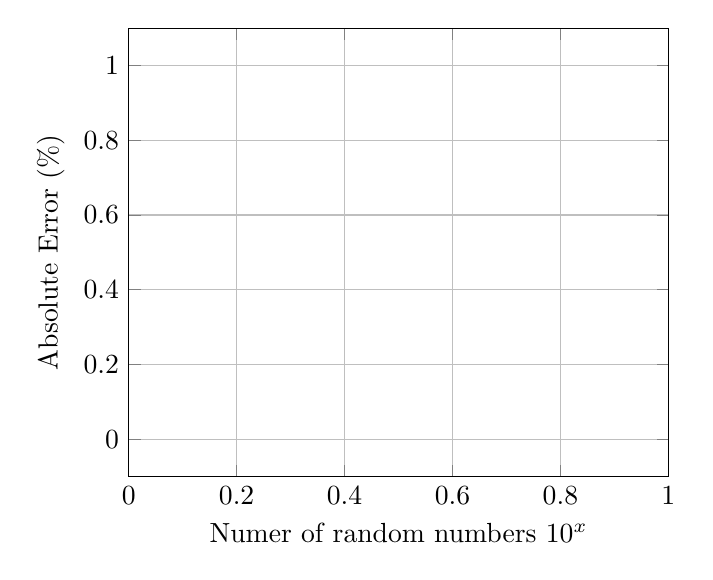
\begin{tikzpicture}
\begin{axis}
[
	xmin=0,   xmax=4,
	grid=major,
	xlabel=Numer of random numbers $10^x$,
	ylabel=Absolute Error (\%)
]
\montecarlo{10}{1}
\montecarlo{100}{2}
\montecarlo{1000}{3}
\end{axis}
\end{tikzpicture}
\caption{The absolute error in percent for various amount of random numbers. One can see that with thousand random numbers the accuracy is quite reasonable. }
\label{fig:monte:carlo}
\end{figure}

\begin{exercise}
Make a list of which C++ features we need to implement the flow chart in Figure~\ref{fig:algorithm:monte}.
\end{exercise}


%----------------------------------------------------------------------------------------
\chapter{$N$-body problems}
%----------------------------------------------------------------------------------------

%----------------------------------------------------------------------------------------
\chapter{One-dimensional heat equation}
%----------------------------------------------------------------------------------------

%----------------------------------------------------------------------------------------
\section{Peridynamics}
%----------------------------------------------------------------------------------------

%----------------------------------------------------------------------------------------
\part{Parallel and distributes computing}
%----------------------------------------------------------------------------------------

%----------------------------------------------------------------------------------------
\chapter{Parallel computing}
%----------------------------------------------------------------------------------------

\section{Shared memory}

\section{Distributed memory}

\part{Introduction: HPX}

\chapter{HPX}

\section{Introduction to HPX}

\section{Parallel algorithms}

\section{Asynchronous programming}

%----------------------------------------------------------------------------------------
%	BIBLIOGRAPHY
%----------------------------------------------------------------------------------------

\chapter*{Bibliography}
\addcontentsline{toc}{chapter}{\textcolor{azure}{Bibliography}} % Add a Bibliography heading to the table of contents

%------------------------------------------------

\section*{Articles}
\addcontentsline{toc}{section}{Articles}
\printbibliography[heading=bibempty,type=article]

%------------------------------------------------

\section*{Books}
\addcontentsline{toc}{section}{Books}
\printbibliography[heading=bibempty,type=book]




%----------------------------------------------------------------------------------------
%	INDEX
%----------------------------------------------------------------------------------------

\cleardoublepage % Make sure the index starts on an odd (right side) page
\phantomsection
\setlength{\columnsep}{0.75cm} % Space between the 2 columns of the index
\addcontentsline{toc}{chapter}{\textcolor{azure}{Index}} % Add an Index heading to the table of contents
\printindex % Output the index

%----------------------------------------------------------------------------------------
%	List of Listings
%----------------------------------------------------------------------------------------

\cleardoublepage % Make sure the index starts on an odd (right side) page
\phantomsection
\addcontentsline{toc}{chapter}{\textcolor{azure}{List of Listings}}
\lstlistoflistings

%----------------------------------------------------------------------------------------
%	List of Figures
%----------------------------------------------------------------------------------------

\cleardoublepage % Make sure the index starts on an odd (right side) page
\phantomsection
\addcontentsline{toc}{chapter}{\textcolor{azure}{List of Figures}}
\listoffigures

%----------------------------------------------------------------------------------------
%	List of Video lectures
%----------------------------------------------------------------------------------------

\chapter*{List of video lectures}
\addcontentsline{toc}{chapter}{\textcolor{azure}{Video lectures}}


\begin{itemize}
\item \href{https://www.youtube.com/watch?v=asGZTCR53KY&list=PL7vEgTL3FalY2eBxud1wsfz8OKvE9sd_z}{C++ Lecture 1 - The Standard Template Library}
\end{itemize}



\end{document}
